\documentclass[10pt]{article}
\usepackage[a4paper]{geometry}
\usepackage{amsmath}
\usepackage{amssymb}
\usepackage{tocbibind}
\usepackage{graphicx}
\usepackage{hyperref}
\usepackage{mdframed}
\usepackage{subfiles}
\usepackage{titlesec}
\usepackage[dvipsnames]{xcolor}

%%%%%%%%%%%%%%%%%%%%%%%%%%%%%%%%%%%%%%%%%%%%%%%%%%%%%%%%%%%%%%%%%%%%%%%% Setups
\newcommand{\Eq}[1]{Equation~\ref{eq:#1}}
\newcommand{\Fig}[1]{Figure~\ref{fig:#1}}

\newenvironment{textbox}[1]
{%
  \mdfsetup{%
    frametitle={\colorbox{white}{\space#1\space}},
    frametitleaboveskip=-\ht\strutbox,
  }
  \begin{mdframed}
}
{
  \end{mdframed}
}

\setlength\parindent{0pt}
\setlength\parskip{1.2ex}

\graphicspath{{./fig/}}

\hypersetup{%
  hidelinks,
  colorlinks,
  citecolor={YellowOrange!85!black},
  linkcolor={Aquamarine!85!black},
  bookmarksopen=true,
  bookmarksnumbered=true,
  linktoc=all,
  pdfauthor=Jihang Li,
}

\title{Notes of ``Human-centric Indoor Scene Synthesis Using Stochastic Grammar''}
\author{Jihang Li}
%%%%%%%%%%%%%%%%%%%%%%%%%%%%%%%%%%%%%%%%%%%%%%%%%%%%%%%%%%%%%%%%%%%%%%%%%%%%%%%

\begin{document}
\maketitle
\tableofcontents

%%%%%%%%%%%%%%%%%%%%%%%%%%%%%%%%%%%%%%%%%%%%%%%%%%%%%%%%%%%%%%%%%%%%%% Abstract
\section*{Abstract}%
\label{sec:abstract}
 Human contexts as contextual relations are encoded by \textbf{Markov Random
 Field (MRF)} on the terminal nodes.

 Distributions are learned from an indoor scene dataset.

 New layers are sampled using \textbf{Monte Carlo Markov Chain (MCMC)}.

 Sampling is based on three criteria:
 %
\begin{enumerate}
  \item Visual realism compare to SOTA room arrangement method.
  \item Accuracy of the affordance maps w.r.t.\ ground-truth.
  \item The functionality and naturalness of synthesized rooms evaluated by
    human subjects.
\end{enumerate}

%%%%%%%%%%%%%%%%%%%%%%%%%%%%%%%%%%%%%%%%%%%%%%%%%%%%%%%%%%%%%%%%%%%%% Chapter 1
\section{Introduction}%
\label{sec:introduction}
Traditional methods of image data collection and labeling limitations:
%
\begin{enumerate}
  \item High-quality ground truths are hard to obtain, as depth and surface
    normal obtained from sensors are always noisy.
  \item Impossible to label certain ground truth information.
  \item Manual labeling of massive ground-truth is tedious and error-prone.
\end{enumerate}

The proposed algorithm is useful for (but not limited to):
%
\begin{enumerate}
  \item Learning and inference for computer vision tasks.
  \item 3D content generation.
  \item 3D reconstruction and robot mappings.
  \item Benchmarking of both low-level and high-level task-planning problems in
    robotics.
\end{enumerate}

Four major difficulties in synthesizing:
%
\begin{enumerate}
  \item The number of pieces may vary in a functional group. (e.g.\ a dinning
    set.)
  \item There is already a quadratic number of object-object relation even if
    only pair-wise relations are considered.
  \item Most object-object relations are not obviously meaningful. (e.g.\ a pen
    and a monitor both on a desk.)
  \item An excessive number of constrains are generated due to the previous
    difficulties.
\end{enumerate}

Contributions:
%
\begin{enumerate}
  \item Jointly model objects, affordances, and activity planning for indoor
    scene configurations.
  \item Provide a general learning and sampling framework for indoor scene
    modeling.
  \item Demonstrate the effectiveness of this structured joint sampling by
    extensive comparative experiments.
\end{enumerate}


%%%%%%%%%%%%%%%%%%%%%%%%%%%%%%%%%%%%%%%%%%%%%%%%%%%%%%%%%%%%%%%%%%%%% Chapter 2
\section{Representation of Indoor Scenes}%
\label{sec:representation}
An attributed S-AOG combines:
%
\begin{enumerate}
  \item A \textbf{probabilistic context free grammar (PCFG)}.
  \item Contextual relations defined on an MRF, i.e.\ the horizontal links
    among the nodes.
\end{enumerate}

An S-AOG is defined as a 5-tuple: $\mathcal{G} = \langle S, V, R, P, E \rangle$,
where:
%
\begin{itemize}
  \item $S$: the root node of the scene grammar
  \item $V$: the vertex set
    \begin{itemize}
      \item $V = V_{NT} \cup V_T$
      \item $V_{NT} = V^{And} \cup V^{Or} \cup V^{Set}$\footnote{$V^{Set}$: A
          set of Or-nodes serving as child branches are grouped by an And-node,
          and each child branch may include different numbers of objects.}
      \item $V_T = V^r_T \cup V^a_T$
        \begin{enumerate}
          \item Regular terminal node: $v \in V^r_T$, represents a spatial
            entity in a scene with \textbf{internal attributes} of object sizes
            $(w, l, h)$, and \textbf{external attributes} $A_{ext}$ of
            object position $(x, y, z)$ and orientation ($x - y$ plane)
            $\theta$ and sampled human positions.
          \item Address terminal node: $v \in V^a_T$, encodes interactions that
            only occur in a certain context but a absent in all others.
        \end{enumerate}
    \end{itemize}
  \item $R$: the production rules
  \item $P$: the probability model
  \item $E$: the contextual relations, $E = E_f \cup E_o \cup E_g \cup E_r$
    \begin{itemize}
      \item $E_f$: relations among furniture
      \item $E_o$: relations between supported objects and their supporting
        objects
      \item $E_g$: relations in a functional pair
      \item $E_r$: relations between furniture and the room
    \end{itemize}
\end{itemize}

\setcounter{figure}{2}
\begin{figure}[!htpb]
  \centering
  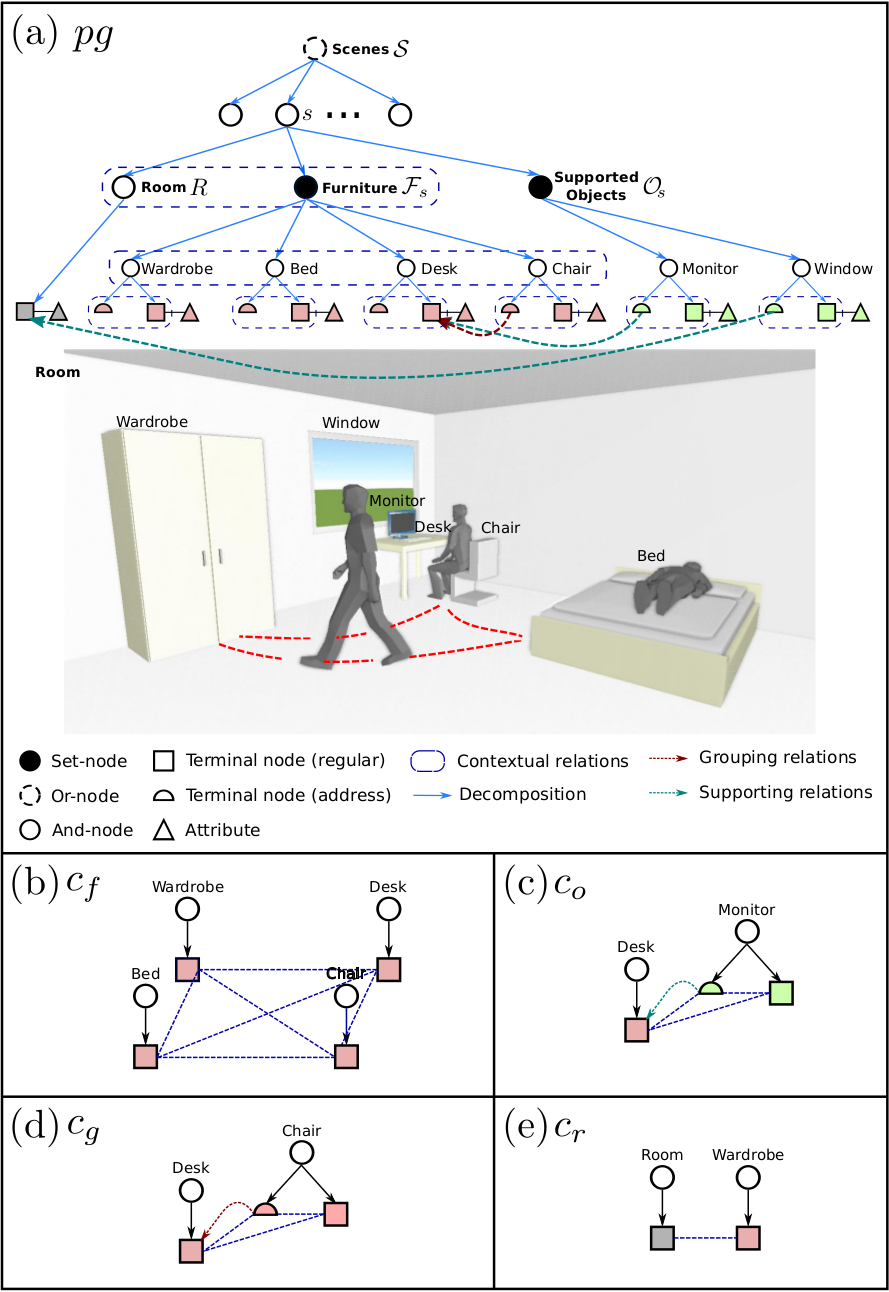
\includegraphics[width=0.6\linewidth]{fig_3.png}
  \caption{(a) A simplified example of a parse graph of a bedroom. The terminal
    nodes of the parse graph form an MRF in the terminal layer. Cliques are
    formed by the contextual relations projected to the terminal layer.
    Examples of the four types of cliques are shown in (b) --- (e),
    representing four different types of contextual relations.}%
  \label{fig:3}
\end{figure}


\newpage
%%%%%%%%%%%%%%%%%%%%%%%%%%%%%%%%%%%%%%%%%%%%%%%%%%%%%%%%%%%%%%%%%%%%% Chapter 3
\section{Probabilistic Formulation of S-AOG}%
\label{sec:formulation}
The \textbf{prior probability} of $pg$ generated by an S-AOG parameterized by
$\Theta$ is formulated as a Gibbs distribution:
%
\begin{align}
  p(pg \vert \Theta) &= \frac{1}{Z} \{-\mathcal{E}(pg \vert \Theta)\} \label{eq:1} \\
                     &= \frac{1}{Z} \{-\mathcal{E}(pt \vert \Theta) - \mathcal{E}(E_{pt} \vert \Theta)\}, \label{eq:2}
\end{align}
%
where:
%
\begin{itemize}
  \item $\mathcal{E}(pg \vert \Theta)$: the energy function of a $pg$
  \item $\mathcal{E}(pt \vert \Theta)$: the energy function of a $pt$
  \item $\mathcal{E}(E_{pt} \vert \Theta)$: the energy term of the contextual
    relations
\end{itemize}
%
$\mathcal{E}(pt \vert \Theta)$ can be decomposed into:
%
\begin{align}
  \label{eq:3}
  \mathcal{E}(pt \vert \Theta) = \underbrace{\sum_{v \in V^{Or}} \mathcal{E}^{Or}_{\Theta}(v) + \sum_{v \in V^{Set}} \mathcal{E}^{Set}_{\Theta}(v)}_{\text{non-terminal nodes}} + \underbrace{\sum_{v \in V^r_T} \mathcal{E}^{A_{in}}_{\Theta}(v)}_{\text{terminal nodes}},
\end{align}
%
where the choice of the child node of an $v \in V^{Or}$ and the child branch of
a $v \in V^{Set}$ follows \textbf{different multinomial distributions}. $A_{in}$
of terminal nodes follows a non-parametric probability distribution learned by
\textbf{kernel density estimation}.

$\mathcal{E}(E_{pt} \vert \Theta)$ combines the potentials of the 4 types of
cliques, integrating human attributes and $A_{ex}$ of $V^r_T$:
%
\begin{align}
  p(E_{pt} \vert \Theta) &= \frac{1}{Z} \exp \{-\mathcal{E}(E_{pt} \vert \Theta)\} \label{eq:4} \\
                         &= \prod_{c \in C_f} \phi_f(c) \prod_{c \in C_o} \phi_o(c) \prod_{c \in C_g} \phi_g(c) \prod_{c \in C_r} \phi_r(c). \label{eq:5}
\end{align}
%

\textbf{Human Centric Potential Functions:}
%
\begin{itemize}
  \item $\phi_f(c)$\footnote{The subscripts, $f$, $o$, $g$, and $r$, hold the
    similar meanings as those in the contextual relation notations.}:
    %
    \begin{align}
      \label{eq:6}
      \phi_f(c) = \frac{1}{Z} \exp\{-\lambda_f \cdot \langle \sum_{f_i \neq f_j} l_{col}(f_i, f_j), l_{ent}(c) \rangle\},
    \end{align}
    %
    where:
    %
    \begin{itemize}
      \item $c = \{f_i\} \in C_f$ includes all the $V_T$ representing furniture.
      \item $\lambda_f$ is a weight vector.
      \item $\langle \cdot, \cdot \rangle$ denotes a vector.
      \item $l_{col}(f_i, f_j)$ (cost function) is the overlapping volume of
        the two pieces of furniture, serving as the \textbf{penalty of
        collision}.
      \item $l_{ent}(c) = -H(\Gamma) = \sum_i p(\gamma_i) \log p(\gamma_i)$
        yields better utility of the room space by sampling human trajectories,
        where $\Gamma$ is the set of planned trajectories in the room, and
        $H(\Gamma)$ is the \textbf{entropy}. The probability map is first
        obtained by planning a trajectory $\gamma_i$ from the center of every
        piece of furniture to another one using \textbf{bi-directional
        rapidly-exploring random tree (RRT)}, which forms a heatmap.
        $H(\Gamma)$ is computed from the heatmap as shown in \Fig{4}.
        %
        \begin{figure}[!htpb]
          \centering
          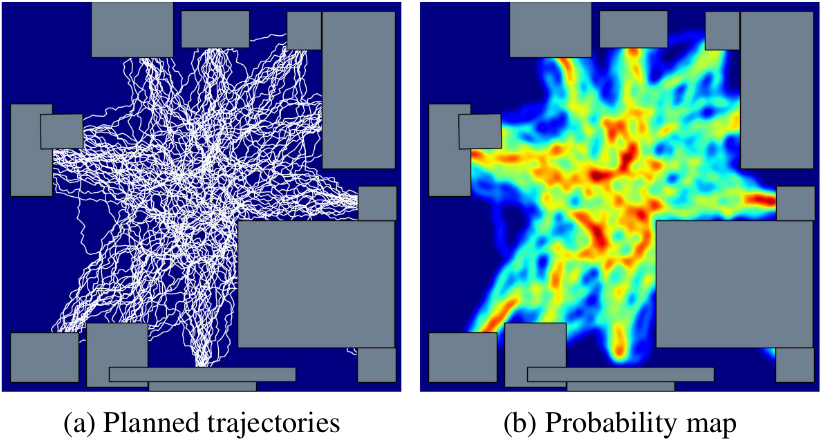
\includegraphics[width=0.6\linewidth]{fig_4.png}
          \caption{Given a scene configuration, we use bi-directional RRT to
            plan from every piece of furniture to another, generating a human
            activity probability map.}%
          \label{fig:4}
        \end{figure}
        %
    \end{itemize}
  \item $\phi_o(c)$:
    %
    \begin{align}
      \label{eq:7}
      \phi_o(c) = \frac{1}{Z} \exp\{-\lambda_o \cdot \langle l_{num}(f, o), l_{add}(a) \rangle\},
    \end{align}
    %
    where:
    %
    \begin{itemize}
      \item $c = \{f, a, o\} \in C_o$ includes a supported object $o \in V_T$,
        $a \in V^a_T$ connected to $o$, and a furniture $f \in V_T$ pointed by
        $a$.
      \item $l_{num}(f, o)$ defines the human usability cost --- a favorable
        human position should enable agent to access or use both the furniture
        and the object. To compute, human position $h^o_i$ are first sampled
        based on position, orientation, and the affordance map of $o$. Given an
        $f$:
        %
        \begin{align}
          \label{eq:8}
          l_{num}(f, o) = \max_i p(h^o_i \vert f).
        \end{align}
        %
      \item $l_{add}(a)$ is the \textbf{negative log probability} of a
        $v \in V^a_T$, treated as a certain $v \in V^r_T$, following a
        multinomial distribution.
    \end{itemize}
  \item $\phi_g(c)$:
    %
    \begin{align}
      \label{eq:9}
      \phi_g(c) = \frac{1}{Z} \exp\{-\lambda_g \cdot \langle l_{num}(f_i, f_j), l_{add}(a) \rangle\},
    \end{align}
    %
    where $c = \{f_i, a, f_j\} \in C_g$ consists of terminal nodes of a core
    functional $f_i$, pointed by the $a$ of an associated $f_j$.
\end{itemize}

\textbf{Other Potential Functions:}
%
\begin{itemize}
  \item $\phi_r(c)$:
    %
    \begin{align}
      \label{eq:10}
      \phi_r(c) = \frac{1}{Z} \exp\{-\lambda_r \cdot \langle l_{dis}(f, r), l_{ori}(f, r) \rangle\},
    \end{align}
    %
    where:
    %
    \begin{itemize}
      \item $c = \{f, r\} \in C_r$ includes a furniture $f \in V_T$ and a room
        $r$.
      \item $l_{dis}(f, r) = -\log p(d \vert \Theta)$ is the distance cost
        function, in which $d \sim \ln \mathcal{N}(\mu, \sigma^2)$ is the
        distance between the $f$ and the nearest wall.
      \item $l_{ori}(f, r) = -\log p(\theta \vert \Theta)$, where
        $\theta \sim p(\mu, \kappa) = \frac{e^{\kappa \cos (x - \mu)}}{2 \pi I_0(\kappa)} $
        is the relative orientation between the model and the nearest wall
        modeled by a \textbf{von Mises distribution}.
    \end{itemize}
\end{itemize}


%%%%%%%%%%%%%%%%%%%%%%%%%%%%%%%%%%%%%%%%%%%%%%%%%%%%%%%%%%%%%%%%%%%%% Chapter 4
\section{Learning S-AOG}%
\label{sec:learning}
Use SUNCG dataset as training data and collect the statistics of:
%
\begin{itemize}
  \item room types
  \item room sizes
  \item furniture occurrences
  \item furniture sizes
  \item relative distances
  \item orientations between furniture and walls
  \item furniture affordance
  \item grouping occurrences
  \item supporting relations
\end{itemize}
%
The parameters $\Theta$ of the probability model $P$ can be learned in a
\textbf{supervised} way by \textbf{maximum likelihood estimation (MLE)}.

\textbf{Weights of Loss Functions:} Recall
%
\begin{align}
  p(E_{pt} \vert \Theta) &= \frac{1}{Z} \{-\mathcal{E}(E_{pt} \vert \Theta)\} \label{eq:11} \\
                         &= \frac{1}{Z} \{-\langle \lambda, l(E_{pt}) \rangle\}, \label{eq:12}
\end{align}
%
where:
%
\begin{itemize}
  \item $\lambda$: weight vector.
  \item $l(E_{pt})$: the loss vector given by the 4 types of potential functions.
\end{itemize}

To learn the weight vector, the standard MLE maximizes the average
log-likelihood:
%
\begin{align}
  \label{eq:13}
  \mathcal{L}(E_{pt} \vert \Theta) = -\frac{1}{N} \sum^N_{n=1} \langle \lambda, l(E_{pt_n}) \rangle - \log Z.
\end{align}
%
which is usually maximized by following the gradient:
%
\begin{align}
  \frac{\partial \mathcal{L}(E_{pt} \vert \Theta)}{\partial \lambda} &= -\frac{1}{N} \sum^n_{N=1} l(E_{pt_n}) - \frac{\partial \log Z}{\partial \lambda} \label{eq:14} \\
                                                                     &= -\frac{1}{N} \sum^n_{N=1} l(E_{pt_n}) - \frac{\partial \log \sum_{pt} \exp \{-\langle \lambda, l(E_{pt}) \rangle\}}{\partial \lambda} \label{eq:15} \\
                                                                     &= -\frac{1}{N} \sum^n_{N=1} l(E_{pt_n}) + \sum_{pt} \frac{1}{Z} \exp \{-\langle \lambda, l(E_{pt}) \rangle\} l(E_{pt}) \label{eq:16} \\
                                                                     &= -\frac{1}{N} \sum^n_{N=1} l(E_{pt_n}) + \frac{1}{\widetilde{N}} \sum^{\widetilde{N}}_{\widetilde{n}=1} l(E_{pt_{\widetilde{n}}}), \label{eq:17}
\end{align}
%
where ${\{E_{pt_{\widetilde{n}}}\}}_{\widetilde{n}=1, \ldots, \widetilde{N}}$
is the set of synthesized examples from the current model.

\begin{textbox}{\textit{Original Texts}}
It is usually computationally infeasible to sample a Markov chain that burns
into an \textit{equilibrium distribution} at every iteration of gradient
ascent. Hence, instead of waiting for the Markov chain to converge, we adopt
the \textbf{contrastive divergence (CD)} learning that follows the gradient of
difference of two divergences:
\end{textbox}
%
\begin{align}
  \label{eq:18}
  \text{CD}_{\widetilde{N}} = \text{KL}(p_0 \| p_{\infty}) - \text{KL}(p_{\widetilde{n}} \| p_{\infty}),
\end{align}
%
where $\text{KL}(p_0 \| p_{\infty})$ is the \textbf{Kullback-Leiber} divergence
between the data distribution $p_0$ and the model distribution $p_{\infty}$,
and $p_{\widetilde{n}}$ is the distribution obtained by a Markov chain started
at the data distribution and run for a small number $\widetilde{n}$ of steps.
In this paper, $\widetilde{n} = 1$.

The gradient of CD is given by:
%
\begin{align}
  \frac{\partial \text{CD}_{\widetilde{N}}}{\partial \lambda} &= \frac{1}{N} \sum^N_{n=1} l(E_{pt_n}) - \frac{1}{\widetilde{N}} \sum^{\widetilde{N}}_{\widetilde{n}=1} l(E_{pt_{\widetilde{n}}}) \label{eq:19} \\
                                                              &- \frac{\partial p_{\widetilde{n}}}{\partial \lambda} \frac{\partial \text{KL}(p_{\widetilde{n}} \| p_{\infty})}{\partial p_{\widetilde{n}}} \nonumber,
\end{align}
%
where the third term can be ignored.

Finally, the weight vector is learned by gradient descent computed by
generating a small number $\widetilde{N}$ of examples from the Markov chain:
%
\begin{align}
  \label{eq:20}
  \lambda_{t+1} &= \lambda_t - \eta_t \frac{\partial \text{CD}_{\widetilde{N}}}{\partial \lambda} \\
                &= \lambda_t + \eta_t \left( \frac{1}{\widetilde{N}} \sum^{\widetilde{N}}_{\widetilde{n}=1} l(E_{pt_{\widetilde{n}}}) - \frac{1}{N} \sum^N_{n=1} l(E_{pt_n}) \right)
\end{align}

\textbf{Branching Probabilities:} The MLE of the branch probabilities $\rho_i$
of $V^{Or}$, $V^{Set}$, and $V^a_T$ is the frequency of each alternative
choice: $\rho_i = \#(v \rightarrow u_i) / \sum^{n(v)}_{n=1} \#(v \rightarrow u_j)$.

\textbf{Grouping Relations:} The grouping relations are \textbf{hand-defined}.
The probability of occurrence is learned as a multinomial distribution, and the
supporting relations are \textbf{automatically} extracted from SUNCG\@.

\textbf{Room Size and Object Sizes:} Of which the distribution is learned as
a non-parametric distribution. The size information is extracted from the 3D
models inside SUNCG, and then a non-parametric distribution is fit using
\textbf{kernel density estimation}. The distances and relative orientations of
the furniture and objects to the nearest wall are computed and fitted into a
\textbf{log normal} and a mixture of \textbf{von Mises distributions},
respectively.

\textbf{Affordance:} Affordance maps of all the furniture and supported objects
are learned by computing the heatmap of possible human positions. These
position include annotated humans, and we assume that the center of chairs,
sofas, and beds are positions that humans often visit. By accumulating the
relative positions, we get reasonable affordance maps as non-parametric
distributions as shown in \Fig{5}.
%
\begin{figure}[!htpb]
  \centering
  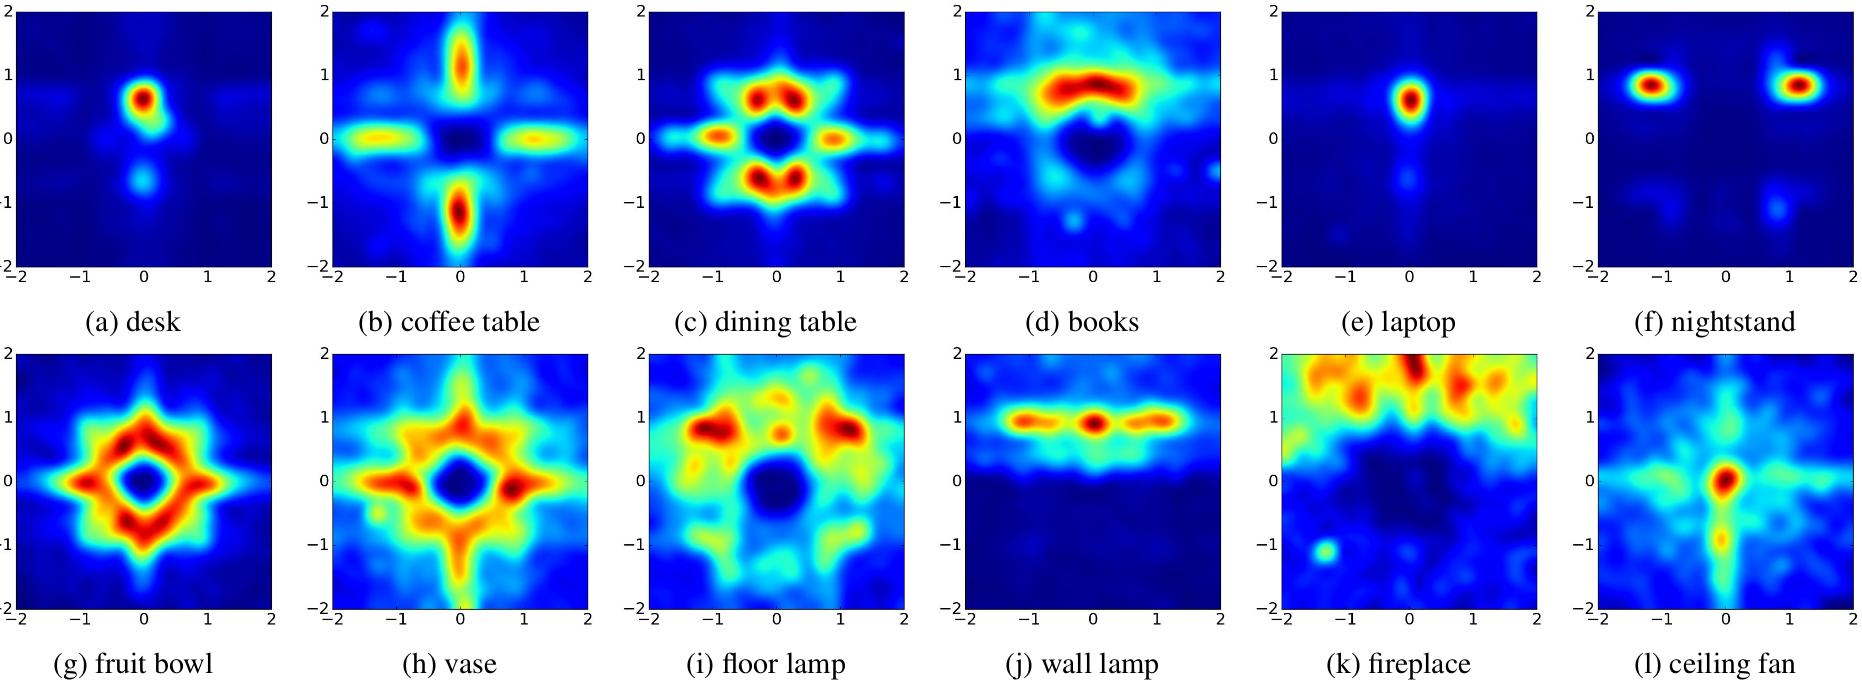
\includegraphics[width=0.9\linewidth]{fig_5.png}
  \caption{Examples of the learned affordance maps. Given the object positioned
    in the center facing upwards, i.e., coordinate of (0, 0) facing direction
    (0, 1), the maps show the distributions of human positions. The affordance
    maps accurately capture the subtle differences among desks, coffee tables,
    and dining tables. Some objects are orientation sensitive, e.g., books,
    laptops, and night stands, while some are orientation invariant, e.g.,
    fruit bowls and vases.}%
  \label{fig:5}
\end{figure}


%%%%%%%%%%%%%%%%%%%%%%%%%%%%%%%%%%%%%%%%%%%%%%%%%%%%%%%%%%%%%%%%%%%%% Chapter 5
\section{Synthesizing Scene Configurations}%
\label{sec:synthesiz}
Synthesizing scene configurations is accomplished by:
%
\begin{itemize}
  \item Sampling a $pg$ from the prior probability $p(pg \vert \Theta)$ defined
    by the S-AOG\@.
  \item The structure of a $pt$ and $A_{in}$ (sizes) can be sampled from the
    closed-form distributions or non-parametric distributions.
  \item For $A_{ex}$ (positions and orientations), a \textbf{Markov Chain
    Monte Carlo (MCMC)} sampler is utilized to draw a typical state in the
    distribution:
    %
    \begin{enumerate}
      \item Directly sample the structure of $pt$ and $A_{in}$: (i) sample the
        child node for $V^{Or}$; (ii) determine the state of each child branch
        of $V^{Set}$; (iii) for each $V^r_T$, sample the sizes and human
        positions from learned distributions.
      \item Use an MCMC scheme to sample the values of $V^a$ and $A_{ex}$ by
        making proposal moves. A sample will be chosen after the Markov chain
        converges.
    \end{enumerate}
    %
\end{itemize}

Two types of Markov chain dynamics $q_i, i=1,2$ are designed and used at random
with probabilities to make proposal moves:
%
\begin{itemize}
  \item $q_1$: \textbf{translation} of objects. It chooses a $v \in V^r_T$, and
    samples a new position based on the current position
    $x \rightarrow x + \delta x$, where $\delta x$ follows a
    \textbf{bivariate normal distribution}.
  \item $q_2$: \textbf{rotation} of objects. It chooses a $v \in V^r_T$, and
    samples a new orientation based on the current orientation
    $\theta \rightarrow \theta + \delta \theta$, where $\delta \theta$
    follows a \textbf{normal distribution}.
\end{itemize}

Adopting the \textbf{Metropolis-Hastings} algorithm, the proposed new
$pg\prime$ is accepted according to the acceptance probability:
%
\begin{align}
  \alpha(pg\prime \vert pg, \Theta) &= \min(1, \frac{p(pg\prime \vert \Theta) p(pg \vert pg\prime)}{p(pg\vert \Theta) p(pg\prime \vert pg)}) \label{eq:22} \\
                                    &= \min(1, \exp(\mathcal{E}(pg \vert \Theta) - \mathcal{E}(pg\prime \vert \Theta))), \label{eq:23}
\end{align}
%
\begin{textbox}{\textit{Original Texts}}
where the proposal probability rate is canceled since the proposal moves are
symmetric in probability. A \textbf{simulated annealing} scheme is adopted to
obtain samples with high probability as shown in \Fig{6}.
\end{textbox}
%
\begin{figure}[!htpb]
  \centering
  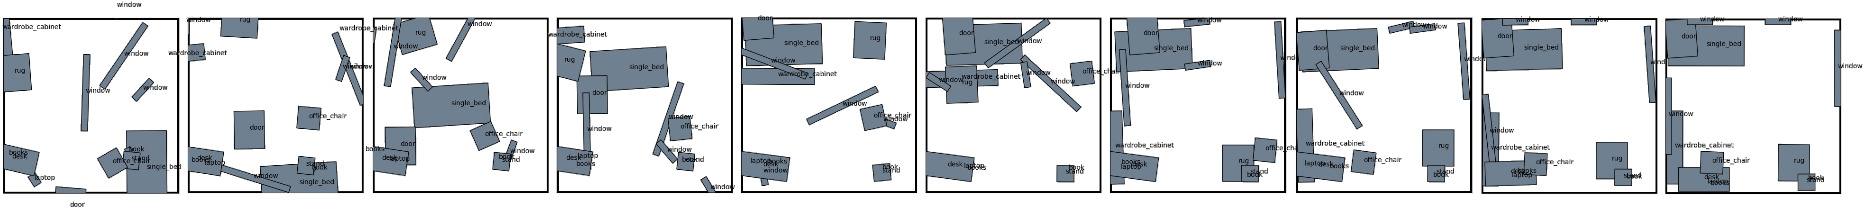
\includegraphics[width=0.9\linewidth]{fig_6.png}
  \caption{MCMC sampling process (from left to right) of scene configurations
    with simulated annealing}%
  \label{fig:6}
\end{figure}


%%%%%%%%%%%%%%%%%%%%%%%%%%%%%%%%%%%%%%%%%%%%%%%%%%%%%%%%%%%%%%%%%%%%% Chapter 6
\section{Experiments}%
\label{sec:experiments}
(Omitted.)


\newpage
%%%%%%%%%%%%%%%%%%%%%%%%%%%%%%%%%%%%%%%%%%%%%%%%%%%%%%%%%%%%%%%%%%%%% Chapter 7
\section{Conclusion}%
\label{sec:conclusion}
\begin{textbox}{\textit{Original Texts}}
We propose a novel general framework for human-centric indoor scene synthesis
by sampling from a spatial And-Or graph. The experimental results demonstrate
the effectiveness of our approach over a large variety of scenes based on
different criteria. In the future, to synthesize physically plausible scenes, a
physics engine should be integrated. We hope the synthesized data can
contribute to the broad AI community
\end{textbox}

\end{document}
